%Tex root = ProbabilitàEStatistica.tex

\chapter{Calcolo combinatorio}

\section{Permutazione}
Consideriamo tre palline colorate.

\begin{figure}[H]
    \centering
    
\includegraphics[width=0.2\textwidth]{images/palline-permutazione.png}
    \caption{palline colorate}
\end{figure}

Disegniamo ora, tutte le possibile sequenze ordinate che si possono ottenere con le tre palline.

\begin{figure}[H]
    \centering
    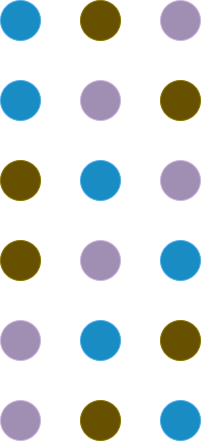
\includegraphics[width=0.2\textwidth]{images/permutazione.png}
    \caption{permutazioni di tre palline}
\end{figure}

\Definizione{permutazione semplice}{
    Le \textbf{permutazioni semplici} sono tutte le possibili sequenze ordinate di n oggetti.
    \begin{equation*}
        p_n = n \cdot (n - 1) \cdot (n - 2) \dots \cdot 1 = n!
    \end{equation*}
}

\vario{Esercizio 1}{
In quanti modi si possono disporre 10 persone in 10 sedie?

\medskip
\noindent
\[
\boxed{10} \cdot \boxed{9} \cdot \boxed{8} \cdot \boxed{7} \cdot \boxed{6} \cdot \boxed{5} \cdot \boxed{4} \cdot \boxed{3} \cdot \boxed{2} \cdot \boxed{1} = 10!
\]
}

\vario{Esercizio 2}{
Calcolare il numero degli anagrammi della parola "CUORE".

\medskip
\noindent
\[
    p_5 = \boxed{5} \cdot \boxed{4} \cdot \boxed{3} \cdot \boxed{2} \cdot \boxed{1} = 5!
\]
}

\vario{Esercizio 3}{
Calcolare il numero degli anagrammi della parola "PICCHE".

\medskip
In questo caso il numero totale di permutazioni non può essere calcolato come la semplice sequenza ordinata scambiando le varie lettere della parola picche, perchè la c è presente due volte (pi\textbf{c}che = pic\textbf{c}he).

Il numero totale di permutazioni (in caso di ripetizioni di alcuni oggetti):
\begin{equation*}
    p_n = \frac{\text{tot. permutazioni tutti n oggetti}}{\text{tot. permutazioni oggetti ripetuti}} = \frac{6!}{2!} = \frac{6 \cdot 5 \cdot 4 \cdot 3 \cdot \cancel{2!} }{\cancel{2!}} = 90
\end{equation*}
}

\section{Dispozione}
Consideriamo una gara di corsa con 9 partecipanti.

\begin{figure}[H]
\centering
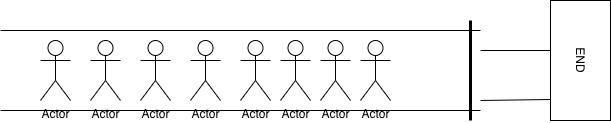
\includegraphics[width=0.3\textwidth]{images/gara.png}
\caption{gara di corsa}
\end{figure}

Quanti podi (3 persone) si possoono creare da un gruppo di 9 persone?

\begin{figure}[H]
\centering
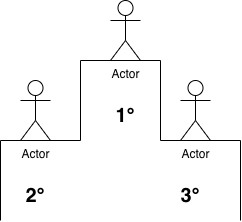
\includegraphics[width=0.2\textwidth]{images/disposizione.png}
\caption{disposizione}
\end{figure}

Per il primo posto abbiamo 9 possibilità, per il secondo posto 8 possibilità e per il terzo posto 7 possibilità.

\Definizione{disposizione semplice}{
Una \textbf{disposizione semplice} è un sotto-insieme di k elementi diversi tra loro selezionati da un insieme di partenza avente n elementi.

\[
    \begin{aligned}
    D_{n,k} &= n \cdot (n - 1) \cdot (n - 2) \dots (n - k + 1) \cdot \textcolor{orange}{\frac{(n - k) \cdot (n - k - 1) \dots 2 \cdot 1}{(n - k) \cdot (n - k - 1) \dots 2 \cdot 1}}\\
            &= \frac{n!}{(n - k)!}
    \end{aligned}
\]

\noindent\rule{\linewidth}{0.4pt}
\textbf{N.B.} Nelle disposizioni è importante l'ordine!
}

\osservazione{
Due disposizioni sono diverse se cambia \textbf{almeno} un elemento, oppure se gli stessi elementi compaiono in ordine differente.
}

\vario{Esercizio 1}{
Quanti numeri di 3 cifre distinte si possono fare utilizzando solo cifre dispari?

\medskip
$cifre_{dispari} = 1, 3, 5, 7, 9$

\[
    \boxed{5} \cdot \boxed{4} \cdot \boxed{3}
\]

\begin{equation*}
    D_{5,3} = \frac{5!}{2!} = \frac{5 \cdot 4 \cdot 3 \cdot \cancel{2!}}{\cancel{2|}} = 60
\end{equation*}
}

\vario{Esercizio 2}{
Calcolare la soluzione di:
\begin{equation*}
    3D_{x,4} = D_{x,5}
\end{equation*}

\[
    \begin{aligned}
    D_{x,4} = \frac{x!}{(x - 4)!} = \frac{x \cdot (x-1) \cdot (x-2) \cdot (x-3) \cdot \cancel{(x-4)!}}{\cancel{(x-4)!}}\\
    D_{x,5} = \frac{x!}{(x - 5)!} = \frac{x \cdot (x-1) \cdot (x-2) \cdot (x-3) \cdot (x-4) \cdot \cancel{(x-5)!}}{\cancel{(x-5)!}}
    \end{aligned}
\]

\osservazione{
    $ x \geq 5$
}

\[
    \begin{aligned}
    3x(x-1)(x-2)(x-3) &= x(x-1)(x-2)(x-3)(x-4) \\
    3 &= x-4 \\
    x &= 7
    \end{aligned}
\]
}

\section{Combinazione}

\Definizione{combinazione semplice}{
Una \textbf{combinazione semplice} è un sotto-insieme di k elementi distinti estratti da un insieme di partenza di n elementi.

\begin{equation*}
    C_{n,k} = \binom{n}{k} = \frac{n!}{k! \cdot (n - k)!}
\end{equation*}
}